\section{The E-HSFP Framework}
\label{sec:method}

Figure~\ref{fig:hsfp_framework} shows how the upper tiers prepare their training inputs. At each interface, the system replays stored moments, masks source outputs, optionally accumulates statistics at the edge, and aggregates the resulting summaries. The learner then samples Gaussian features and trains its model component. Model, optimizer, and synthesis state persist across phases. The system maintains one record bank per interface and one reliability network shared by the upper tiers. \reviewblue{Each subsection below implements one operator of the pipeline~\eqref{eq:synthesis_pipeline}: replay $\mathsf R_\alpha$ (Section~\ref{sec:memory}), masking $\mathsf D_{p_{\mathrm{train}}}$, accumulation $\mathsf K_\gamma$, and aggregation $\mathsf A_\phi$ (Section~\ref{sec:reliability}), and synthesis $\mathsf G$ (Section~\ref{sec:lowrank}).} The defaults below describe the implementation. Section~\ref{sec:experiments} identifies the reported settings of the historical runs.

\begin{figure*}[t]
    \centering
    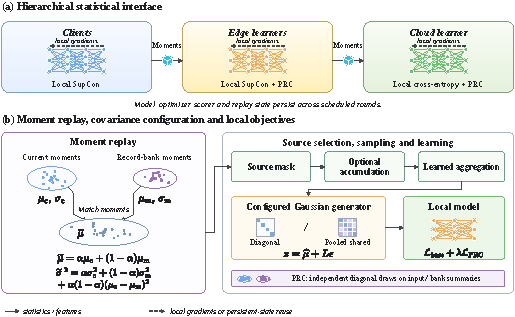
\includegraphics[width=\linewidth]{figures/method.drawio.pdf}
    \caption{Hierarchical training and upper-tier processing in \ehsfp{}. (a) Clients train on local examples; edge and cloud components train on synthesized features. Class-wise moments connect the tiers, with additional scatter for optional shared-covariance synthesis. (b) Moment replay, source masking, optional accumulation, and learned aggregation prepare the Gaussian training inputs. Classification supports diagonal or full shared covariance with diagonal fallback. PRC compares independent diagonal draws from input-side and memory summaries. Solid arrows denote statistics or feature flow. Dashed arrows denote local gradients or persistent-state reuse. The replay equation omits numerical jitter. Separate model synchronization and the ISIC-2018 supervised decoder stage are omitted.}
    \label{fig:hsfp_framework}
\end{figure*}

\subsection{Prototype Memory and Moment Replay}
\label{sec:memory}

The client--edge bank stores summaries from clients, and the edge--cloud bank stores summaries from edges. Each record contains class moments, support count, source identifier, generation round, age, and retrieval score. New summaries enter the bank before replay and keep their generation timestamps. Capacity enforcement favors more recent records. If a per-class cap applies, exceeding it removes a record of the highest age for that class. By default, each bank holds up to 500 records with a 20-round retention limit and no separate per-class cap.

For each class, the implementation retrieves up to $K_{\mathrm{mem}}=5$ records by default to form the memory moments $(\pmu_{\mathrm m}^{(j)},\psigma_{\mathrm m}^{(j)})$. It aggregates them with the total-variance rule in~\eqref{eq:agg_mean_var}, using normalized retrieval scores or uniform weights if their sum is below $\zeta$. The implemented retrieval scores stay at one and are separate from the learned aggregation scores. Record order breaks ties, and retrieval may include summaries that arrived in the current round.

When replay is enabled and $\alpha<1$, each existing source $\ell$ combines its current moments with the memory moments for each class represented in both sets. The combined moments are
\begin{equation}
\begin{split}
 \widetilde{\pmu}_{\ell}^{(j)}
 &=\alpha\pmu_{\mathrm c,\ell}^{(j)}
 +(1-\alpha)\pmu_{\mathrm m}^{(j)},\\
 (\widetilde{\psigma}_{\ell}^{(j)})^2
 &=\alpha(\psigma_{\mathrm c,\ell}^{(j)})^2
 +(1-\alpha)(\psigma_{\mathrm m}^{(j)})^2\\
 &\quad+\alpha(1-\alpha)
 (\pmu_{\mathrm c,\ell}^{(j)}-\pmu_{\mathrm m}^{(j)})^2+\zeta .
\end{split}
\label{eq:memory_mixture}
\end{equation}
Squares are coordinate-wise. The mixing coefficient $\alpha\in[0,1]$ weights the current moments, with a default of $0.3$ and $\alpha=1$ bypassing replay. With replay active, a class represented on only one side uses that side's moments. Equation~\eqref{eq:memory_mixture} gives the mixture mean and coordinate-wise variance with added jitter $\zeta$, which we set to $\zeta=10^{-8}$ as a numerical safeguard. The generator samples from a single Gaussian with these moments. \reviewblue{Proposition~\ref{prop:replay_drift} bounds the drift that this mixing adds when the current moments are fresh.} Replay can add a class found only in memory to an existing source output. An empty packet collection gives replay no source output to augment. The controller ages records and removes expired ones at the end of the round, so a delayed arrival may be used before this step.

\subsection{Source Masking and Learned Aggregation}
\label{sec:reliability}
\label{sec:dropout}

After replay, the mask independently marks each source output for removal with probability $\dropoutp_{\mathrm{train}}$. If it marks every output in a nonempty collection, the learner restores one chosen uniformly at random. A single source is always retained, and an empty collection stays empty. This restoration step makes the final retention indicators generally dependent. \reviewblue{Proposition~\ref{prop:masking_coverage} gives the resulting class-loss probability in closed form.} A masked source can already have contributed to the record bank. The retained sources can still omit classes or yield too few synthetic features for a valid minibatch.

Optional edge accumulation combines the retained outputs into one effective source. For each class, it maintains a decayed support total $A_0$ and support-weighted sums $A_1$ and $A_2$ of first and second raw moments. With decay $\gamma$, the update is
\begin{equation}
 (A_0,A_1,A_2)\leftarrow
 \gamma(A_0,A_1,A_2)
 +\sum_{\ell}n_\ell
 \bigl(1,\pmu_\ell,\psigma_\ell^2+\pmu_\ell^2\bigr).
 \label{eq:accumulated_moments}
\end{equation}
Missing or zero support receives unit weight. The accumulator reconstructs the mean as $A_1/A_0$ and the coordinate-wise variance as $\max\{A_2/A_0-(A_1/A_0)^2,\zeta\}$. It rounds the effective counts for use as metadata. The same decay applies to available scatter statistics and their degrees of freedom. The edge sees one effective source after accumulation. Contributions decay without a hard age cutoff.

For class $j$, let $\mathcal S^{(j)}$ index the resulting sources. The scorer uses support, spread $s_\ell=\|\psigma_\ell^{(j)}\|_2$, age $a_\ell$, and distance $d_\ell$ from the arithmetic mean of the source means for that class. Its six inputs are normalized log support, normalized spread, normalized age, normalized distance, a constant one, and a second copy of normalized log support. The support feature is $\log(1+n_\ell)/\log(1+\max\{1,n_{\max}\})$, with missing support set to zero. The spread and distance denominators are their respective class maxima, each floored at $\zeta$. The age denominator is the class maximum age, floored at one. A $6$--$32$--$32$--$1$ ReLU network with sigmoid output produces the source scores $f_\phi(v_\ell^{(j)})$. The corresponding weights are
\begin{equation}
 \omega_\ell^{(j)}
 =\frac{f_\phi(v_\ell^{(j)})}
 {\max\{\sum_{q\in\mathcal S^{(j)}}f_\phi(v_q^{(j)}),\zeta\}} .
 \label{eq:reliability_weight}
\end{equation}
The weights sum to one when the score sum is at least $\zeta$. When the floor is active, their sum is below one. The implementation uses these safeguarded weights in the class moment estimates
\begin{equation}
\begin{split}
 \widehat{\pmu}^{(j)}
 &=\sum_{\ell\in\mathcal S^{(j)}}\omega_\ell^{(j)}\pmu_\ell^{(j)},\\
 (\widehat{\psigma}^{(j)})^2
 &=\sum_{\ell\in\mathcal S^{(j)}}\omega_\ell^{(j)}
 \bigl[(\psigma_\ell^{(j)})^2
 +(\pmu_\ell^{(j)}-\widehat{\pmu}^{(j)})^2\bigr]+\zeta .
\end{split}
\label{eq:agg_mean_var}
\end{equation}
Count-weighted aggregation instead uses normalized support counts, with uniform weights when all counts are zero. The legacy uniform rule averages coordinate-wise variances without the between-source mean term. Comparisons with this rule therefore change both weighting and variance construction.

After round-end bank maintenance, the implementation trains the shared scorer using targets computed from record metadata. Each class in the client bank with at least two records contributes one mean-squared-error training step. The target averages $\min(n/100,1)$, $(1+s)^{-1}$, and $(1+a)^{-1}$, using $0.5$ for the support term when $n\le0$. The scorer defaults to Adam with learning rate $10^{-3}$ and weight decay $10^{-4}$. Its learned scores serve as proxies for source reliability. \reviewblue{Each of the three contributions is bounded in $[0,1]$. Their equal coefficients give support, compactness, and recency the same nominal scale, while 100 is a fixed support scale at which the count contribution saturates. These are implemented heuristic choices, not calibrated coefficients or consequences of the convergence analysis; the bootstrap target is not derived from downstream task loss and has no optimality guarantee. Proposition~\ref{prop:weighting_shift} shows that its effect on the synthetic mean is confined to classes whose sources disagree.}

\subsection{Gaussian Feature Synthesis}
\label{sec:lowrank}

Diagonal synthesis applies~\eqref{eq:prelim_synthesis} to the aggregated moments. Classification additionally supports a full covariance shared across classes. Each reporting source supplies within-class scatter
$S_\ell=\sum_i(x_{\ell i}-\pmu_\ell^{(y_{\ell i})})(x_{\ell i}-\pmu_\ell^{(y_{\ell i})})^\top$,
where $x_{\ell i}$ is a feature vector and $y_{\ell i}$ is its class label. The source also reports its sample count $N_\ell$ and represented-class count $C_\ell$. Pooling the source statistics gives
\begin{equation}
 \nu=\sum_\ell(N_\ell-C_\ell),\qquad
 \Sigma_0=\frac{\sum_\ell S_\ell}{\nu},\quad \nu>1.
 \label{eq:pooled_covariance}
\end{equation}
The instantaneous estimate is
$\Sigma=(1-\beta)\Sigma_0+\beta\operatorname{diag}(\Sigma_0)$,
where $\beta=\max\{0,1-\nu/(2d)\}$.
When accumulation is enabled, the covariance uses the ratio of accumulated scatter to the corresponding accumulated degrees of freedom.
\reviewblue{Shrinkage toward a diagonal covariance target is a standard stabilization strategy~\cite{schafer2005shrinkage}. Here the target is exactly $\operatorname{diag}(\Sigma_0)$, but the implemented coefficient $\beta=\max\{0,1-\nu/(2d)\}$ is a degrees-of-freedom heuristic rather than the data-estimated coefficient of~\cite{schafer2005shrinkage}. Remark~\ref{rem:scatter_pooling} notes that $\Sigma_0$ omits between-source variation of class means.}

For Cholesky factorization, the learner attempts
$\Sigma+\epsilon_{\mathrm{chol}}s_\Sigma I_d$,
where $s_\Sigma=\max\{\operatorname{tr}(\Sigma)/d,\zeta\}$ and the successive coefficients are $10^{-4},10^{-3},10^{-2},10^{-1}$. The first successful factor yields
\begin{equation}
 z^{(j)}=\widehat{\pmu}^{(j)}+L\epsilon,
 \qquad \epsilon\sim\mathcal N(0,I_d).
 \label{eq:lowrank_synthesis}
\end{equation}
The generator refreshes the covariance before drawing each training pool. A successful factorization uses $LL^\top$ for the main classification pool. The generator uses diagonal synthesis if the full covariance is missing or incompatible, or if all factorization attempts fail. Segmentation and PRC use diagonal synthesis.

\subsection{Local Objectives and Replay Consistency}
\label{sec:regularization}
\label{sec:prc}

Classification clients and edges use supervised contrastive loss~\cite{khosla2020supervised}. Each example supplies two independently transformed views whose outputs are pooled and $\ell_2$-normalized. Other views with the same label form the positive set, and every non-anchor view enters the denominator. Spatial feature maps use crop, flip, and blur transformations. Pooled edge features use additive noise and feature dropout. The client objective can also include a supervised loss. The cloud classification objective uses cross-entropy.

PRC compares the model outputs on pairs of features sampled independently from two class-conditional Gaussians. The first Gaussian uses the replayed source outputs. It averages their means uniformly and uses the root mean square of their standard deviations. The second Gaussian uses moments aggregated from all bank records with their stored scores. At the edge, the learner prepares the first set of moments before local masking and accumulation. At the cloud, it prepares them after masking. The two sets of moments can therefore use some of the same records. For the shared class set $\mathcal C$, let $C=|\mathcal C|>0$ and
$s=\min\{s_{\mathrm{req}},\max(1,\lfloor128/C\rfloor)\}$.
Using $s$ independent pairs from the two diagonal Gaussians for each shared class, the loss is
\begin{equation}
 \mathcal L_{\mathrm{PRC}}
 =\frac{1}{Csd_h}\sum_{j\in\mathcal C}\sum_{a=1}^{s}
 \|h(z_{\mathrm c,a}^{(j)})-h(z_{\mathrm m,a}^{(j)})\|_2^2 .
 \label{eq:prc_loss}
\end{equation}
Here $h$ returns pooled edge representations or cloud logits, and $d_h$ is its output dimension. The loss is zero when $C=0$. The summaries are detached from the computation graph, and gradients pass through both evaluations of $h$. The learner holds the summaries fixed during a phase and samples new pairs for each update that uses PRC. The implementation defaults are $s_{\mathrm{req}}=16$ and $\lambda_{\mathrm{prc}}=0.1$.

The independent draws determine how PRC acts on the outputs. For a fixed deterministic $h$, let $m_b^{(j)}$ and $V_b^{(j)}$ denote its output mean and covariance under side $b\in\{\mathrm c,\mathrm m\}$. Expanding the squared difference gives
\begin{equation}
\begin{split}
 \mathbb E\mathcal L_{\mathrm{PRC}}
 =\frac{1}{Cd_h}\sum_{j\in\mathcal C}
 \bigl(&\|m_{\mathrm c}^{(j)}-m_{\mathrm m}^{(j)}\|_2^2\\
 &+\operatorname{tr}V_{\mathrm c}^{(j)}
 +\operatorname{tr}V_{\mathrm m}^{(j)}\bigr).
\end{split}
\label{eq:prc_decomp}
\end{equation}
For this fixed output map, the expected penalty includes both the discrepancy between the output means and the output variation under each sampling law. \reviewblue{Consequently, $\mathbb E\mathcal L_{\mathrm{PRC}}$ is not minimized by matching the two output laws: even when they coincide, it equals $2(Cd_h)^{-1}\sum_j\operatorname{tr}V^{(j)}$, so PRC also contracts the output variance of $h$ on each class. This contraction may act as a class-compactness regularizer, but it also means that PRC is not a pure consistency penalty.}

The classification upper-tier objectives are
\begin{align}
 \mathcal L_e&=\mathcal L_{\mathrm{SupCon}}
 +\lambda_{\mathrm{prc}}\mathcal L_{\mathrm{PRC}},
 \label{eq:edge_loss}\\
 \mathcal L_g&=\mathcal L_{\mathrm{CE}}
 +\lambda_{\mathrm{prc}}\mathcal L_{\mathrm{PRC},g}.
 \label{eq:cloud_loss}
\end{align}
Source masking changes the synthetic inputs to the base objective. PRC provides the explicit output penalty. For ISIC-2018, a separate supervised stage trains the cloud decoder on image-specific features from frozen upstream modules and target masks using a Dice--focal loss.

\subsection{Processing and Cost}
\label{sec:processing_cost}

Algorithm~\ref{alg:ehsfp} separates preparation of the source summaries from local training. Each phase draws a labeled pool with $n_{\mathrm{syn}}$ examples per active class. The learner reuses this pool for $E$ shuffled epochs and discards incomplete final batches. With $J$ active classes and batch size $B$, the nominal budget is $E\lfloor Jn_{\mathrm{syn}}/B\rfloor$ updates before any execution truncation. The implementation defaults to $n_{\mathrm{syn}}=50$ and $E=10$ and allows each tier to override them. Without a full minibatch, the learner skips optimization. An edge can still extract output summaries from a nonempty pool. A separate draw configured for extraction adds no optimizer steps.

\begin{algorithm}[t]
\caption{Preparation and training at one prototype interface}
\label{alg:ehsfp}
\begin{enumerate}
 \item Insert received summaries into the interface bank, enforce capacity, and moment-mix existing source outputs.
 \item For each addressed learner:
 \begin{enumerate}
  \item Select assigned outputs; apply masking and optional edge accumulation, retaining PRC inputs at the tier-specific point in Section~\ref{sec:prc}.
  \item Aggregate moments, refresh covariance, and draw a labeled pool.
  \item Optimize the local objective within the execution budget; extract edge-output summaries when applicable and retain learning state.
 \end{enumerate}
\end{enumerate}
\end{algorithm}

At the end of each round, after the phases at both interfaces, the controller ages the records, removes expired ones, and trains the shared reliability network once. Model synchronization follows the separate schedules in Section~\ref{sec:formulation}.

For feature dimension $d$, a basic packet contains $2d+1$ scalars per class. Full covariance adds source-level scatter of size $O(d^2)$. The scatter traffic counter assigns $4d(d+1)/2$ bytes to a float32 upper triangle, compared with $4d^2$ bytes for dense storage. Factors require $O(d^2)$ storage, each draw costs $O(d^2)$, and factorization costs $O(d^3)$. The class moments in a bank of $R$ records require $O(Rd)$ storage. Metadata, model synchronization, and segmentation feature/mask transfers add traffic. The estimates describe tensor sizes before serialization and deployment.
